%% The following is a directive for TeXShop to indicate the main file
%%!TEX root =../diss.tex

\chapter{Introduction}
\label{ch:Introduction}

\section{Cancer}

Some facts about prevalence of cancer and poor outcomes, high toxicity to motivate this work.

\subsection{Current therapies}

Numerous advancements in chemotherapies over the past decade have sparked an urgent clinical need for non invasive methods to assess treatment efficacy.
There is a knowledge gap in the use and synergistic combinations of therapies, and many treatment regimens expose patients to higher toxicity than necessary.
Despite known extremes in patient response to treatment - even in cancers of the same type and grade - doses are generally prescribed by success rates of trials in patient populations exhibiting similar disease manifestations.
Each class of drugs has unique modes of action and still, there are no reliable and reproducible methods to assess synergistic benefits of combined therapy regimens~\cite{Zhang:2008ie}.
Traditionally, a prominent measure of treatment response has been to track tumour shrinkage following treatment~\cite{Tuma:2006hx}.
However, it has been shown that tumour shrinkage can take weeks and sometimes even months to manifest~\cite{Brindle:2008jt} and in some cases may not occur at all~\cite{Kitzen:2008un}.
For instance, anti-angiogenic agents typically arrest tumour growth by disrupting existing vasculature or inhibiting new vessel growth.
Despite positive effect, these agents may not necessarily lead to tumour shrinkage.
This mode of drug action is better characterized by assessing tumour vascular function rather than gross changes in physical size.
Development of quantitative and non-invasive methods to assess tumours following therapy continues to be a burgeoning field.Furthermore, there is an urgent need in the drug development and testing community as drugs that fail in the late stages of clinical trials have led to an astronomical rise in the cost of developing drugs.
Lack of any patient stratification techniques to identify potential responders from non-responders is a key reason that drugs fail.
For instance clinical trials targeting hypoxia- a key target for both chemotherapy to improve drug delivery and radiotherapy to increase radiosensitivity - have been conducted without patient selection or stratification based on pre-treatment tumour hypoxia status and therefore include patients with different hypoxic fractions~\cite{Overgaard:2011ji}.
This is at least partially due to an absence of validated methods that can accurately assess the hypoxia status of tumours.The benefits of developing early, non-invasive measures of treatment efficacy are clear for both patients and health care systems.
For patients, if a standard treatment regimen is prescribed and deemed ineffective early, the treatment can be altered and patients can directly benefit from personalized care.
Similarly, with improved patient stratification using non-invasive gross assessments of the tumour status, these patients can avoid receiving potentially ineffective and expensive therapies leading us one stop closer to personalized medicine.
However, the choice of appropriate biomarkers for particular targets remains elusive. 

\subsection{Cancer Biomarkers and targets} There has been considerable interest in predictive biomarkers for early assessment.
Several candidates have appeared and disappeared but in 2000, a seminal paper catalogued a vast array of cancer cell genotypes into ``six essential alterations in cell physiology that collectively dictate malignant growth in tumours''~\cite{Hanahan:2000wo} (figure~\ref{cancerHallmarks}): 1) self-sufficiency in growth signals, 2) insensitivity to growth-inhibitory signals, 3) evasion of programmed cell death, 4) limitless replicative potential, 5) sustained angiogenesis and, 6) tissue invasion and metastasis~\cite{Hanahan:2000wo}.
In 2011, taking into account the progress made over a decade, the framework expanded to inculde four more hallmarks for the next generation~\cite{Hanahan:2011gu}.
Angiogenesis, the 5th hallmark is particularly suitable for consideration in non-invasive imaging techniques, particularly MRI. 

\begin{figure}[htbp]   
 \begin{center}  
 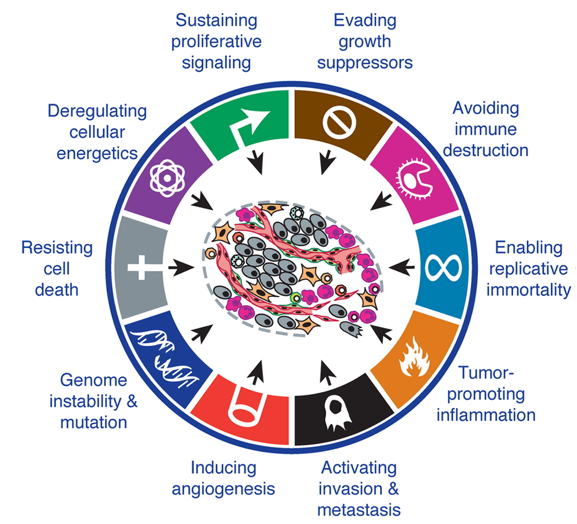
\includegraphics[width=4in]{intro/./intro-images/cancerHallmarks.png}
 \caption{Graphical illustration of the hallmarks of cancer; many of these targets are inaccessible to non-invasive imaging. Figure from the Hanahan group~\cite{Hanahan:2011gu}.}  
 \label{cancerHallmarks}  
 \end{center}
\end{figure}

Angiogenesis, or the formation of new blood vessels from pre-existing ones is a normal and vital process in the body tightly regulated by various cell signalling pathways and growth factors.
In tumours, angiogenesis is a critical step in the growth and spread of tumours as new blood vessels are recruited from the existing vascular network to promote rapidly accelerated and abnormal tumour growth~\cite{Folkman:1990ud}.
Normally, this process is regulated by several angiogenic and antiangiogenic factors such as $\alpha \beta$ integrin, vascular endothelial growth factor (VEGF) and fibroblast growth factor (FGF)~\cite{Laking:2006ij}.
In tumours however, this process is completely deregulated (figure~\ref{tumourVasculature}) and excess production of growth factors from rapidly proliferating tumour cells leads to a drastic increase in vasculogenesis.
These newly formed vessels are unstable and must mature with the addition of pericytes, cells that surround the endothelium providing structural support.
Pericytes are often malformed and poorly distributed in solid tumours contributing to a dysfunctional vascular network.
Vessel growth patterns in tumours are generally accepted to be abnormal with a defective and leaky endothelium~\cite{McDonald:2002ut}.
Irregular diameters of tumour vessels, abnormal branching patterns and leaky vessel walls all contribute to an increase in vessel permeability.
It is estimated that a single hole larger than 0.5$\mu$m in diameter would alter the permeability of that vessel significantly enough to result in solute extravasation to be limited by blood flow~\cite{McDonald:2002ut}.
Disorganized and inefficient blood flow also limits the delivery of macromolecules, such as chemotherapeutic agents via the blood.
Poor perfusion in the tumour due to a disorganized vascular network impairs the delivery of systemic drugs to the whole tumour and ultimately, reduces efficacy. 

%\begin{wrapfigure}{L}{0.65\textwidth} 
\begin{figure}  
 \begin{center}  
 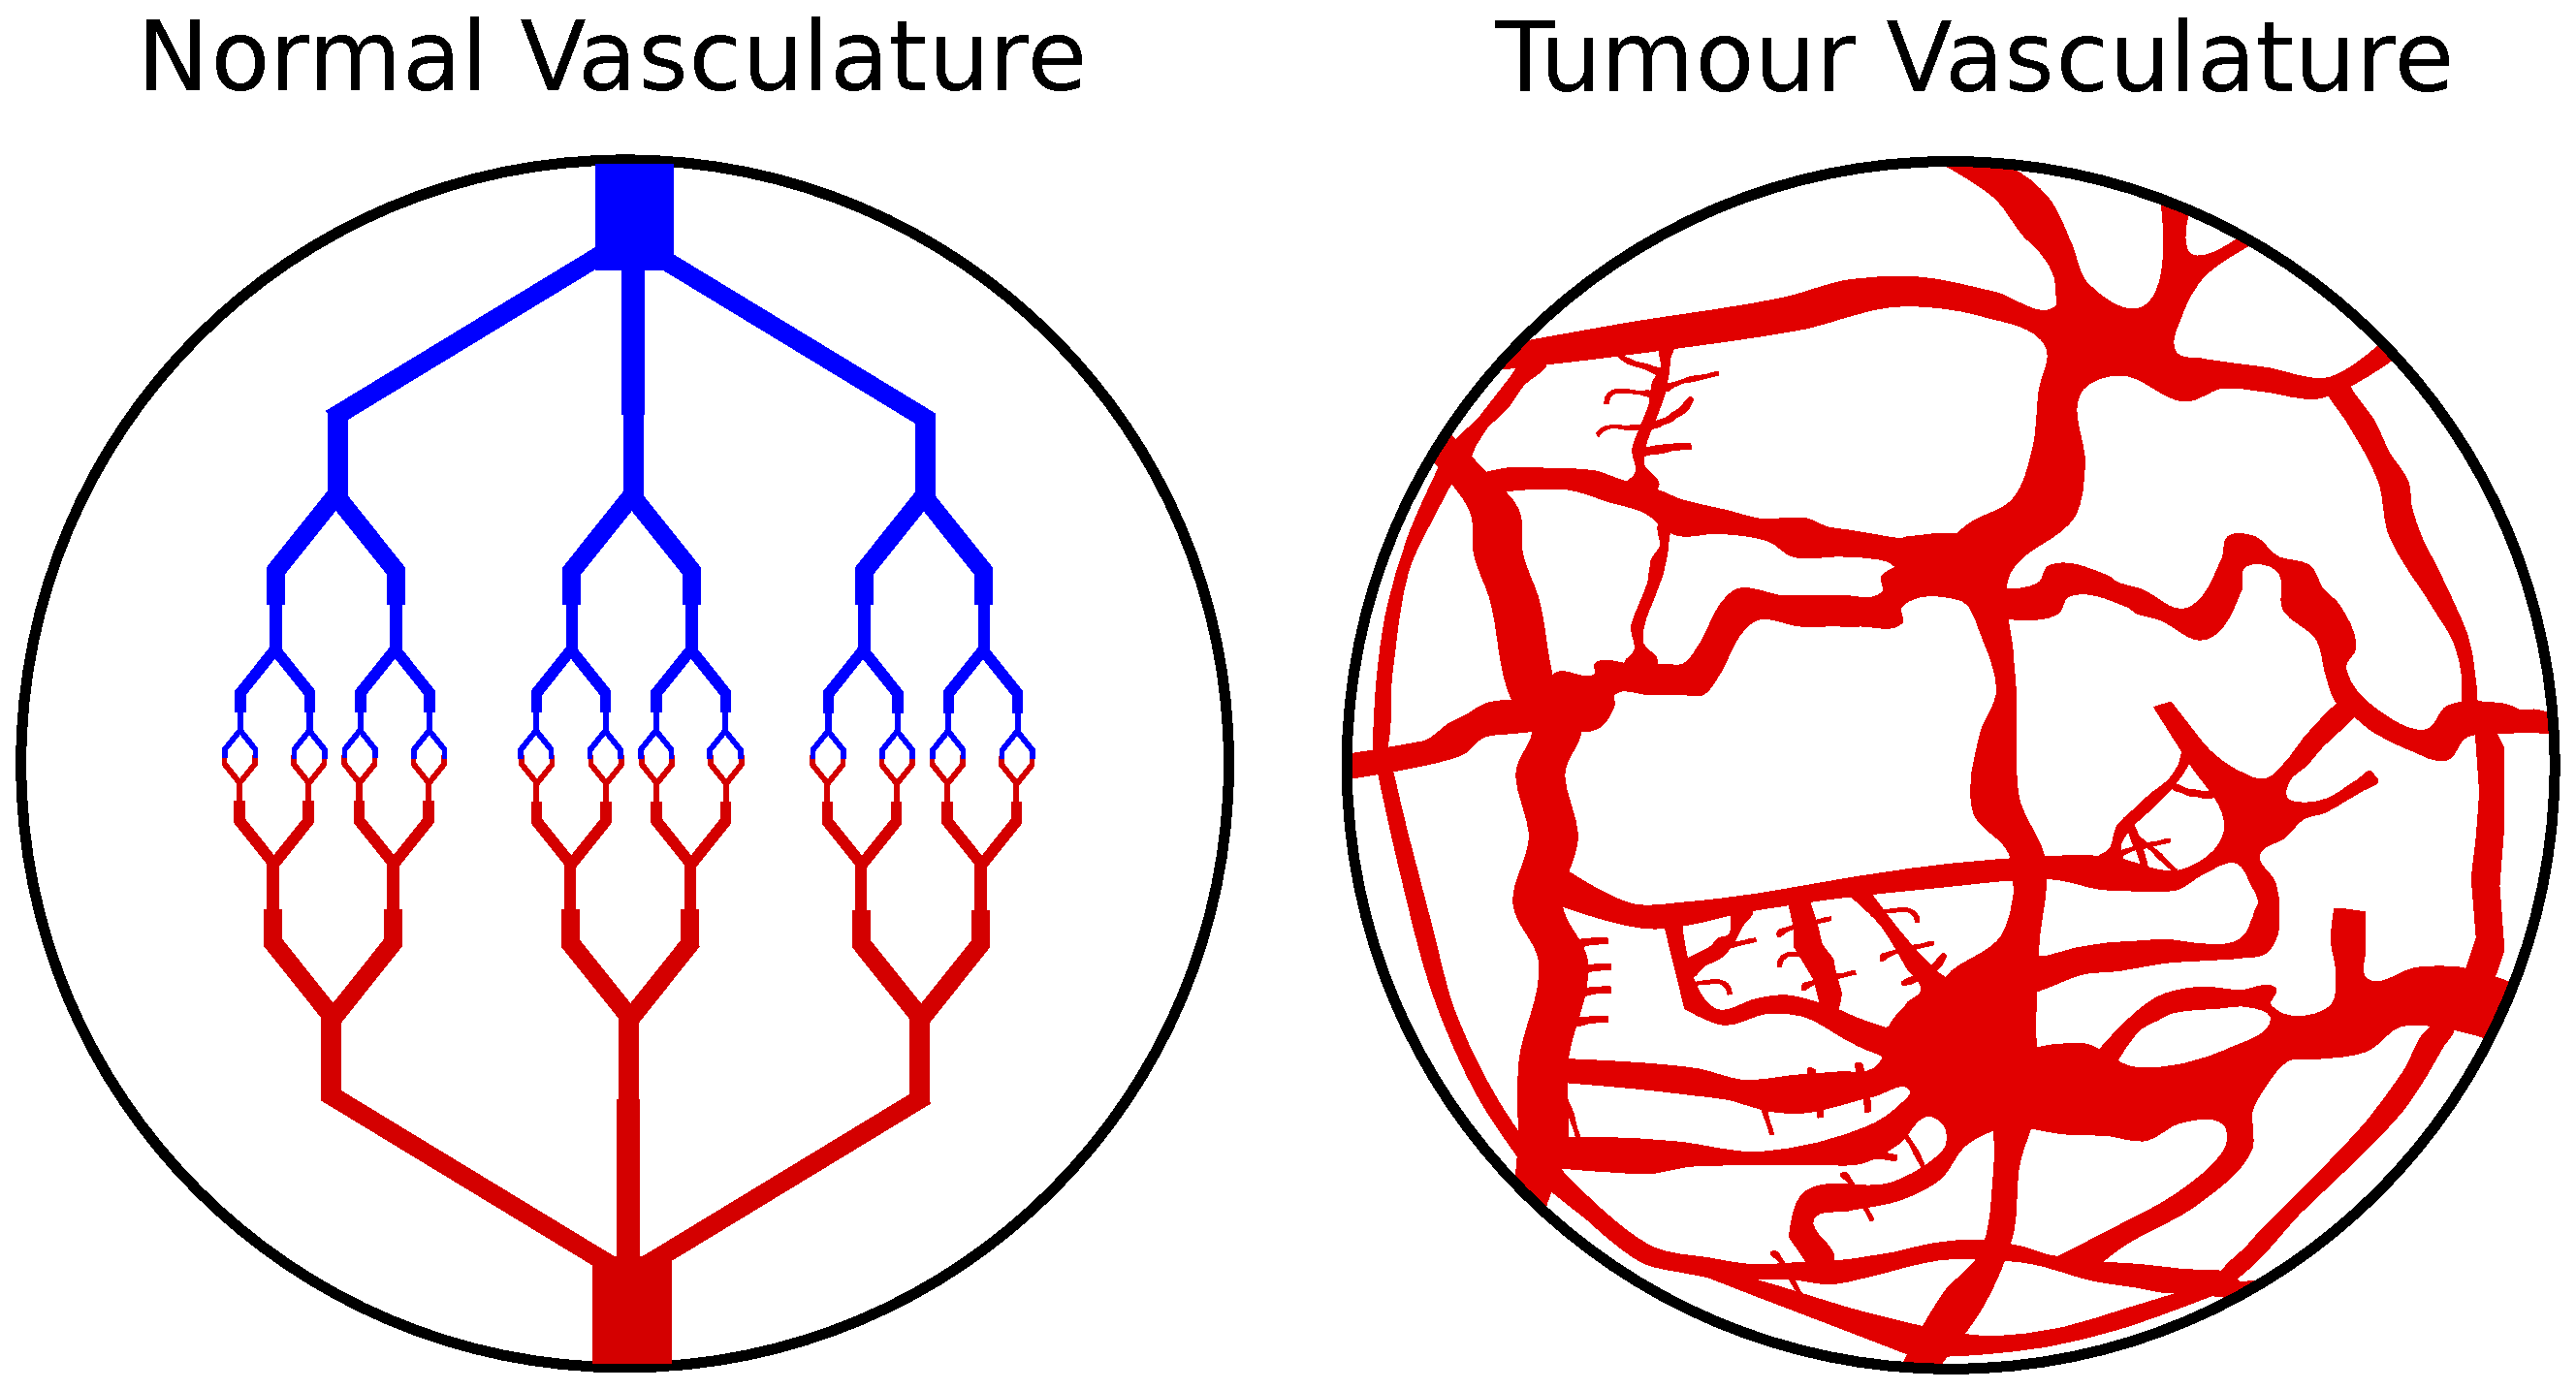
\includegraphics[width=4in]{intro/intro-images/tumourVasculature.pdf}
 \caption{Schematic of the normal tissue (left) and tumour (right) vasculature network. 
 Note the hierarchical structure of oxygenated blood (red) passing through the arteries, arterioles, and deoxygenated blood leaving via the venules, veins. 
 In tumours, this structure is severely compromised and often, no clear flow patterns can be distinguished with many vessels ending in dead ends or looping back onto feeding vessels.}
 \label{tumourVasculature}
 \end{center}
\end{figure}

Several strategies have been proposed to maximize cell kill, including the combination of different therapies (such as radiotherapy and chemotherapy) and agents that ``normalize'' the tumour vasculature and prime them for receiving chemotherapies~\cite{Jain:2005gk}.
Tumour angiogenesis is extremely important in tumour growth, progression and metastasis and is a promising target for novel therapies~\cite{Miles:2000wq}.
For instance, ``measuring'' tumour angiogenesis has the potential to serve as a highly predictive prognostic marker for disease outcome and treatment.
Histology remains the gold standard for angiogenesis detection (microvessel density) but has several critical limitations.
Histology requires biopsy samples and patient comfort aside, biopsies only sample a small fraction of the potentially affected organ.
The lack of functional information from biopsies as well as the practical challenges of obtaining longitudinal biopsy samples make non-invasive imaging a promising technique to complement and potentially reduce unneeded biopsies.

\subsection{Need for non-invasive imaging}
Non-invasive imaging methods are proving indispensable for studying angiogenesis \emph{in vivo} as they provide researchers with quantitative information about blood flow, vascular permeability, vessel density, vessel function and blood volume~\cite{McDonald:2003cm}.
Imaging modalities such as computed tomography (CT), magnetic resonance imaging (MRI), positron emission tomography (PET), single photon emission computed tomography (SPECT) and ultrasound (US), have all been proposed for studying angiogenesis~\cite{Laking:2006ij}.
Each modality is optimal for probing a particular aspect of biomarkers. To study angiogenesis and its effects on tumour growth and treatment response, the tumour environment needs to be probed using tools that assess both the interstitial tumour volume as well as the tumour vasculature.
Nuclear medicine techniques such as PET and SPECT employ radiotracers that can be measured at picomolar concentrations but at a significantly lower spatial resolution.
DCE-MRI and DCE-CT offer similar perfusion measurements (rate of leakage and leakage space) as both rely on the administration of a contrast agent that diffuses from the vasculature.
DCE-CT is advantageous as it has a direct linear relationship between the contrast agent concentration and the image intensity (attenuation numbers, given by Houndsfield Units)~\cite{Cuenod:2006jy}.
The disadvantage of CT however is that it requires ionizing radiation and iodinated contrast agents used in CT have been shown to have lower safety profiles compared to MR contrast agents~\cite{Hasebroock:2009hw}.
MRI can also be used to measure additional information such as diffusion, tissue oxygenation, spectroscopy, chemical exchange and magnetization transfer. 
In this thesis, several techniques will be explored in a bid to improve our understanding of the tumour microenvironment.

\section{Magnetic Resonance Imaging}

%%%%%%%%%%%%%%%%%%%%%

The phenomenon of nuclear magnetic resonance arises in atoms with an odd number of protons and/or an odd number of neutrons. 
In biological specimens, water is the most abundant molecule in the body and the hydrogen atom in water, carbon and many other sources contribute to the overall signal. 

Other MR-active atoms include $^{19}$F, $^{23}$Na and $^{31}$P. 
These atoms possess a property known as spin angular momentum (a quantum-relativistic phenomenon), which arises from the odd number of protons and/or neutrons. 
An ensemble population of atoms possessing angular momentum are referred to as a population of spins. 
In the absence of an external magnetic field, a spin population is expected to point in all  directions and the net magnetic dipole moment sums to zero (figure ~\ref{spinsRest}). 
If the spin population is exposed to an external magnetic field \textbf{B$_0$}, the spins will precess about \textbf{B$_0$} (Fig.~\ref{spinsB0}) and the nuclei will emit energy at a resonant frequency described by the Larmor equation,
		
\begin{equation}
	\omega = \gamma \textbf{B}
\end{equation}
		
%\begin{figure}
%	\centering
%	\includegraphics[width=3in]{chapter1/images/spinsRest.png}
%	\caption[Spins with no magnetic field]{Spins shown here are at rest with no magnetic field applied, leading to a 0 magnetization. 
%Image credit: Hanson et al. (\cite{Hanson:2008tp})}
%	\label{spinsRest}
%\end{figure}

where $\gamma$ is the gyromagnetic ratio, a known constant characteristic for each nucleus. 
Despite the introduction of a strong magnetic field, the energies associated with the orientation of individual spins in \textbf{B$_0$} are much smaller than their thermal energies, so the spins only have a slight tendency to point along the direction of the field~\cite{Hanson:2008tp}. 
Due to the large number of spins the slightly increased tendency of spins to point along the field results in the formation of a longitudinal equilibrium magnetization, \textbf{M} (Fig.~\ref{spinsB0}). 
\todo[backgroundcolor=blue]{Broken reference}
\textbf{M} can be decomposed into two components, the transverse component (M$_{xy}$, initially zero) and the longitudinal component (M$_{z}$, initially a constant $M_0$). 
\textbf{M} is the signal that can be (indirectly) measured in MRI and can be manipulated to generate different contrast between species.
 
The net magnetization vector \textbf{M} arising from spins is many orders of magnitude smaller than the external magnetic field so the MR signal cannot be measured when it is aligned with the external field. 
Application of an RF pulse \textbf{B$_1$} can be interpreted as a torque applied to \textbf{M}, causing it to `tip' down into the transverse plane. 
In the transverse plane, interacting spins exchange energy with both the surrounding spins, as well as the surrounding environment (lattice), and \textbf{M} relaxes back to its equilibrium value. 
Relaxation of the longitudinal component (also called spin-lattice relaxation) of \textbf{M$_0$} from 0 back to the equilibrium value is characterized by the time T$_1$,

\begin{equation}
	M_z = M_z (1-e^{-t/T_1})
	\label{T1}
\end{equation}
		
		Similarly, decay of \textbf{M$_{xy}$} from \textbf{M$_0$} to 0 is characterized by the time T$_2$ (also called spin-spin relaxation).
		
\begin{equation}
		M_{xy} = M_0 e^{-t/T_2}
		\label{T2}
\end{equation}
			
%	\begin{figure}
%	\centering
%	\includegraphics[width=3in]{chapter1/images/spinsB0.png}
%	\caption[Spins in a magnetic field]{In the presence of a magnetic field B$_0$, a longitudinal magnetization forms (vertical arrow) as the spin distribution is skewed slightly towards the direction of the magnetic field. 
%The net magnetization at equilibrium is stationary even though individual spins are precessing around B$_0$. 
%Image credit: Hanson et al. 
%(\cite{Hanson:2008tp})}
%	\label{spinsB0}
%\end{figure}
	
%\begin{figure}
%	\centering
%	\includegraphics[width=3in]{chapter1/images/spinsB0B1.png}
%	\caption[Spins getting tipped with an RF pulse]{The net magnetization vector M$_0$ is tipped to the transverse axis with an RF pulse so the signal can be measured. 
%Image credit: Hanson et al. 
%(\cite{Hanson:2008tp})}
%	\label{spinsB0B1}
%\end{figure}

Signal detection in MRI takes advantage of several principles from electromagnetism: a rotating magnetic moment generates a rotating magnetic field, which is associated with an electric field. 
If a wire coil is placed near the sample, then the electric field induces current in the wire, which can be measured as a voltage. 
As the spins lose coherence, the rotating magnetic moment decreases in amplitude and the induced current also decays. 
The decaying signal is referred to as a free induction decay (FID) and is refocused using gradients and pulses to generate measurable echoes, which then are used to form images.

At a particular magnetic field, T$_1$ and T$_2$ values are intrinsic to each tissue type and depend on local environmental factors such as temperature, proton concentration, and molecular mobility. 
Differences in T$_1$ and T$_2$ values are used to generate contrast between different tissues. 
For example at 3T, brain white matter has a T$_1$ of 1084ms and grey matter has a T$_1$ of 1820 ms~\cite{Stanisz:2005fe}. 
In a T$_1$ weighted image of the brain, imaging parameters are selected such that the T$_1$ recovery curves of the white matter and grey matter are maximally separated and the T$_1$ decay curves are minimally separated. 
The resulting image will distinguish white and grey matter based on their respective T$_1$s, with white matter hyper-intense and grey matter hypo-intense. 
On the other hand, in a T$_2$ weighted image of the brain, white matter is hypo-intense and grey-matter is hyper-intense as white matter T$_2$ decays faster (69ms) than grey matter T$_2$ (99ms). 
Contrast agents in MRI are typically T$_1$ shortening and are designed to increase T$_1$ contrast.

\subsubsection{Dynamic contrast enhanced MRI (\acs{DCE-MRI})}

Tracer kinetic models are often applied to \acs{DCE-MRI} data to extract physiologically relevant information about the microcirculation. 
\acs{DCE-MRI} is frequently used in the clinic to quantitatively asses the kinetics of a contrast agent bolus passing through the body. 
The presence of this agent, typically a paramagnetic species such as Gadolinium, results in a decrease of the longitudinal relaxation time (T$_1$) proportional to the contrast agent concentration. 
In a T$_1$ weighted image then, presence of a Gadolinium-based agent (for e.g., Gd-DTPA) yields an increase in signal intensity. 

Gd-DTPA is a small molecule that readily traverses the endothelium but not the cell membrane~\cite{WalkerSamuel:2006ch}. 
This property provides a mechanism by which the dynamics of vascular leakiness (exchange between capillary bed and the tissue) can be evaluated. 
Choosing a kinetic model to fit the data requires some prior knowledge about the organ or system in question. 
For instance, the presence of the blood brain barrier in the brain dramatically alters the contrast agent kinetics. 
Similarly, in leaky tumours the extravascular contrast agents typically used in \acs{DCE-MRI} leak out (and back in) of vasculature considerably faster than other tissues. 
Sourbron et al. indicate that choice of a tracer kinetic model should provide a link between relevant physiological parameters and measured data~\cite{Sourbron:2011ce}. 
A number of models have been proposed and the most general of these is referred to as the standard two compartment exchange model (2CXM)~\cite{Tofts:1999we} summarized in Fig.~\ref{2CXM}.

\begin{figure}[htbp]
   \centering
   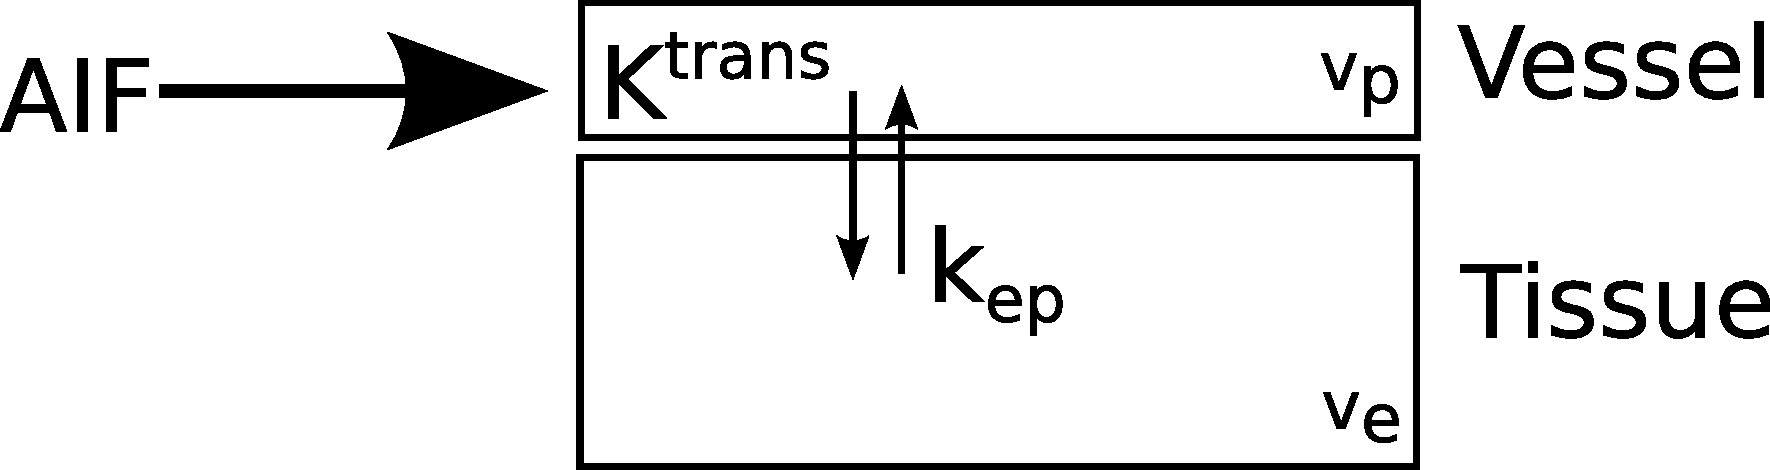
\includegraphics[width=\textwidth]{intro/intro-images/2CXM.pdf}
   \caption[Two compartment exchange model]{Graphical description of the two compartment exchange model. 
An arterial input function (\acs{AIF}) governs the introduction of the tracer in the vascular compartment via a bolus intravenous injection. 
The two transfer constants - \acs{K$^{trans}$} and \acs{k$_{ep}$} -describe the rate at which the tracer is exiting and re-entering, respectively, the vascular component.}
   \label{2CXM}
\end{figure}

A principal assumption of the 2CXM is that the system of interest can be modelled as two compartments, the vasculature (blood plasma) and the extravascular extracellular space (EES). 
A bolus intravenous injection delivers the contrast agent (or tracer) and is characterized by the arterial input function (\acs{AIF}). 
This input function is used to calculate the tracer concentration in the blood plasma over time. 
Because the tracer is small, exchange between the two components occurs readily. 
The rate constant describing the transfer of the tracer from the blood plasma to the EES is termed \acs{K$^{trans}$} and the rate constant in the reverse direction (EES to blood plasma) is referred to as \acs{k$_{ep}$}. 
\acs{K$^{trans}$} and \acs{k$_{ep}$} are related by the volume of the EES,

\begin{equation}
k_{e} = K^{trans} / v_{e},
\label{ke}
\end{equation}

where v$_{e}$ is the volume of the extravascular extracellular space per unit volume of tissue. 
The generalized kinetic model of the tracer in the tissue (C$_t$) is given as a differential equation,

\begin{equation}
\frac{dC_t}{dt} = K^{trans}C_p - k_{ep}C_t,
\label{2CXMeq}
\end{equation}

where C$_p$ is the tracer concentration in the blood plasma and C$_t$, \acs{K$^{trans}$}, \acs{k$_{ep}$} are as described above. 
Solving this differential equation requires an initial condition and the \acs{AIF} provides the tracer concentration at the arrival time, before any exchange in the system occurs (t=0). 
Thus, modelling of \acs{DCE-MRI} data to produce quantitative and physiologically relevant values of \acs{K$^{trans}$}, \acs{k$_{ep}$} and v$_e$ requires an accurate calculation of the \acs{AIF}. 
In clinical studies, determining the \acs{AIF} on a per-patient basis is already accepted as a clinical research standard. 
Direct measurement of the \acs{AIF} is typically performed in an artery within the imaging field of view but such a vessel is not always present and when it is, partial volume, in-flow and signal saturation effects all contribute to confounding \acs{AIF} measurements. 
Direct measurement of the \acs{AIF} is notoriously difficult in small animals using both invasive techniques (small total blood volume prohibits sampling) and non-invasive methods (requires high temporal and spatial resolution to accurately resolve the \acs{AIF}). 
Current \acs{AIF} measurement methods include shunting blood from the carotid artery through a receiver coil and then back into the animal~\cite{Simpson:1999vl} and using a separate receiver coil around the chest~\cite{Pickup:2009ce} or tail~\cite{McIntyre:2004eh}. 
Alternate strategies include using a published population \acs{AIF} from the literature or assuming a mathematical function that models the physiology~\cite{Yankeelov:2006dr}. 
Unfortunately, these strategies are wrought with pitfalls as the inter-subject variability of the \acs{AIF} may be significant and parameters may vary up to 30\% depending on the selected \acs{AIF}~\cite{Simpson:1999vg}. 
In particular for pre-clinical studies, published \acs{AIF}s are not representative of all mouse models as considerable physiological changes exist between species~\cite{Simpson:1999vg}. 
Needless to say, these techniques are all complex, invasive, time consuming and resource intensive and ultimately, add another dimension to the project. 
In this study, we have chosen a model-free approach to analyzing \acs{DCE-MRI} data. 
The leading candidate for model-free analysis is the initial area under the enhancement curve (\acs{AUC}). 
This parameter can be interpreted as a measure of the amount of contrast agent delivered to and retained by the tumour in a specific time period~\cite{Baert:2011uc}. 
An example of a typical \acs{DCE-MRI} enhancement curve with \acs{AUC}$_{60}$ shaded in red is shown in Fig.~\ref{sampleMRcurve}.

%%%%%%%%%%%%%%%%%%%%%%%%

\subsection{T$_1$}
\subsection{T$_2^*$}

\subsection{Contrast mechanisms}
Split into two groups - there are others, but this is what's relevant for this thesis.

Talk about relaxivity and tumbling, water protons.

\subsubsection{Low-MW Agents}
\begin{itemize}
\item Gd-DTPA
\item Modeling (Tofts)
\end{itemize}

\subsubsection{High-MW Agents}
\begin{itemize}
\item Dextran based agents
\item Relaxivity
\end{itemize}

\subsection{Oxygen as a contrast agent}
	\subsection{Theory}

To explore the mechanism of action for the OE-MRI signal, it is useful to first understand the delivery of oxygen from inspired air to tissues. 
The primary mode of oxygen delivery to tissue is the haemoglobin (Hb) molecule as it carries and delivers 98\% of the oxygen in the body. 
Over 250 million Hb molecules are found in a typical red blood cell and each Hb molecule has four binding sites for oxygen molecules. 
The binding affinity for ${O_2}$ drastically increases for subsequent oxygen molecules that bind to Hb as the conformation of the Hb molecule changes to increase binding affinity for the next oxygen, a phenomenon called cooperativity. 
Similarly, when the local environment of the Hb molecule changes such that ${O_2}$ needs to be released, the reverse conformational changes occur so a proportionately lower drop in oxygen tension is required to release the next ${O_2}$ molecule. 
The dissociation of oxygen from haemoglobin molecules is tightly regulated and well described by the oxygen-haemglobin dissociation curve (figure~\ref{HBdis}).

	\begin{figure}
		\begin{center}
		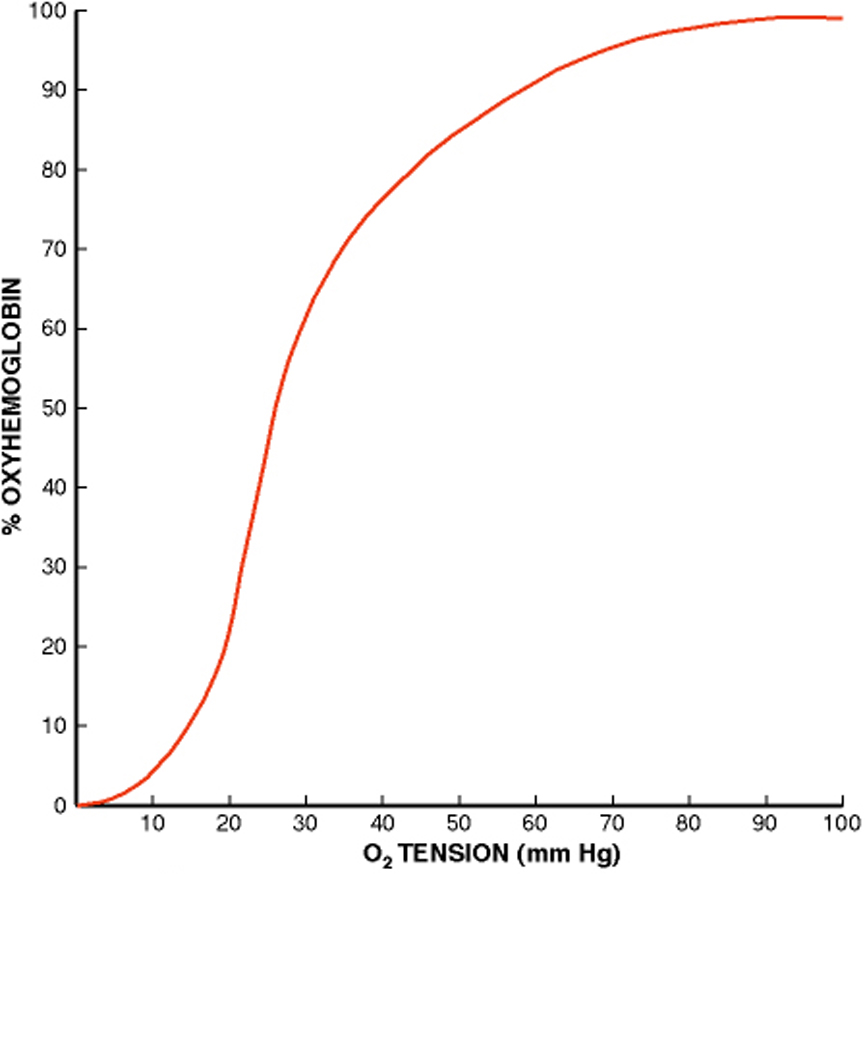
\includegraphics[width=\textwidth]{./intro/intro-images/HBdis.png}
		\caption{Sigmoidal curve illustrating the relationship between the haemoglobin saturation (y-axis) and the oxygen tension (x-axis). Note that the curve is very steep in the middle but it takes a large increase in oxygen tension to bind the last ${O_2}$ and similarly, a large decrease in oxygen tension to release the last  ${O_2}$~\cite{GomezCambronero:2001hu}.}
		\label{HBdis}
		\end{center}
	\end{figure}	

	Next, let's trace the oxygenated blood: upon inspiration of atmospheric air (p$_{O_2}$ = 160 mmHg), gas exchange in the pulmonary capillary beds occurs in the alveoli of the lungs~\ref{mmhg}.
Incoming venous blood with a low oxygen tension (p$_{O_2}$ = 40 mmHg) is oxygenated as haemoglobin molecules readily bind available oxygen. 
As the oxygenated blood leaves the alveoli and moves through the systemic arteries, it has an oxygen tension of 100 mmHg. 
The oxygenated blood then travels from the arteries to the systemic capillary bed, the local oxygen tension drops from 100 to 40 mmHg and the Hb molecule undergoes a structural change releasing a molecule of ${O_2}$ from its first binding site.  
The second release of the oxygen molecule occurs when the tension drops to 26mmHg~\cite{GomezCambronero:2001hu}. 
The third and fourth molecules are released with consecutively smaller drops in oxygen tension as low oxygen tension indicates an oxygen starved environment. This important feature of Hb (cooperativity) ensures that small changes in p$_{O_2}$ have the right effect in the right places. 
For instance, in the lung small changes should not affect the release of ${O_2}$ as tight binding is required so Hb can bind the ${O_2}$ needed to supply all the tissues. 
Conversely, small changes in p$_{O_2}$ in capillary beds should result in easy release of ${O_2}$ so it can easily diffuse to oxygen-starved tissues. 
Practically however, it is important to note that Hb molecules never release all four of the bound oxygen.

	\begin{figure}
		\begin{center}
		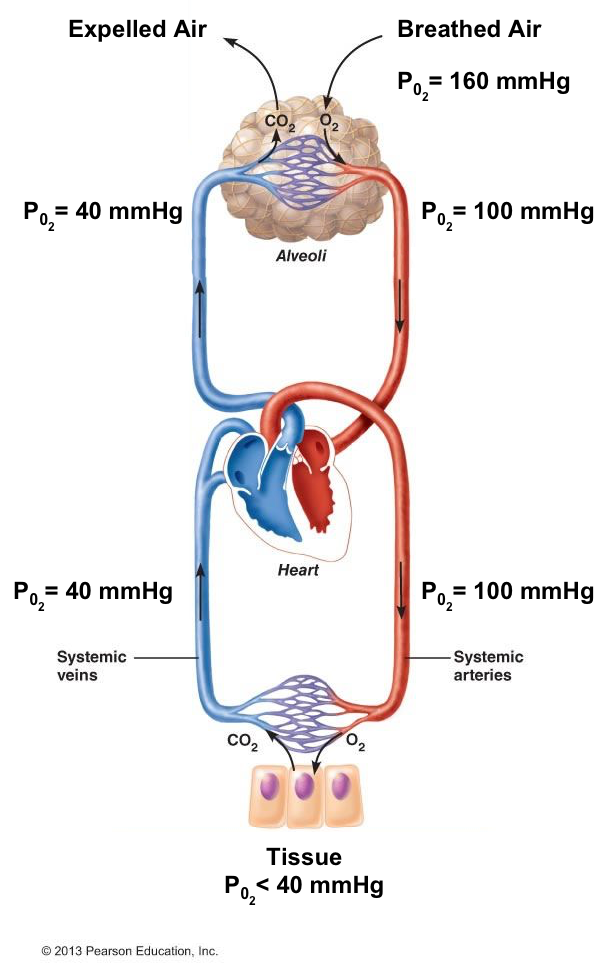
\includegraphics[width=\textwidth]{./intro/intro-images/mmHg.png}
		\caption{A schematic of the oxygen/Hb transport mechanism through the system blood stream. Photo credit: Pearson Education, Inc. 2013}
		\label{mmhg}
		\end{center}
	\end{figure}

\subsubsection{Origin of the OE-MRI Signal}

Oxygen is a paramagnetic molecule because it has two unpaired electrons so it is widely assumed that the dominating effect in the OE-MRI signal is a T$_1$ decrease after concentrated oxygen gas (100\% O$_2$) is breathed in~\cite{OConnor:2016ee,Linnik:2014hf}. 
The excess oxygen travels through the blood stream dissolved in plasma and diffuses through the vessel walls and dissolves in interstitial tissue fluid (figure~\ref{oemri}).
The net increase in dissolved oxygen results in a dramatic and measurable decrease in T$_1$. 
This change is reversed soon after the patient is switched back to breathing atmospheric air as excess oxygen is expelled or metabolized. 
In tumour regions that are perfused (i.e regions that already have a high Hb-O saturation) will see a measurable decrease in T$_1$. 
The perfused regions that do not show a decrease in T$_1$ must therefore be hypoxic~\cite{OConnor:2016ee}. 
Importantly, OE-MRI does not yield any information about unperfused regions and in that region, there are likely to be pockets of viable (but hypoxic) tissue.

The oxygen status of healthy tissue is fairly well regulated in normal tissue and every cell in the body is at most 150$\mu$m away from a blood vessel. 
In tumours however, the vascular network is chaotic and the growth patterns of vessels are abnormal leading to a defective and leaky endothelium~\cite{McDonald:2002}. 
Irregular diameters of tumour vessels, abnormal branching patterns and leaky vessel walls all contribute to an increase in vessel permeability and pockets of hypoxic tissue. 
Unfortunately in hypoxic tissue the oxygen status cannot be well characterized as many factors can influence the oxygen dissociation curve including temperature, pH, and carbon dioxide concentration - all factors that persist unregulated in tumour hypoxic tissue. 
Furthermore, these hypoxic regions are heterogeneous, transient, and drastically differ between tumour models. 
Thanks to some excellent work with spectral imaging using an implanted window chamber in mice, it is known that upon breathing 100\% oxygen, the Hb saturation in the tumour vascular network increases from 20-30\% up to 70-80\% while the Hb saturation in the normal vascular network does not change appreciably~\cite{Sorg:2008eg}.

	\begin{figure}
		\begin{center}
		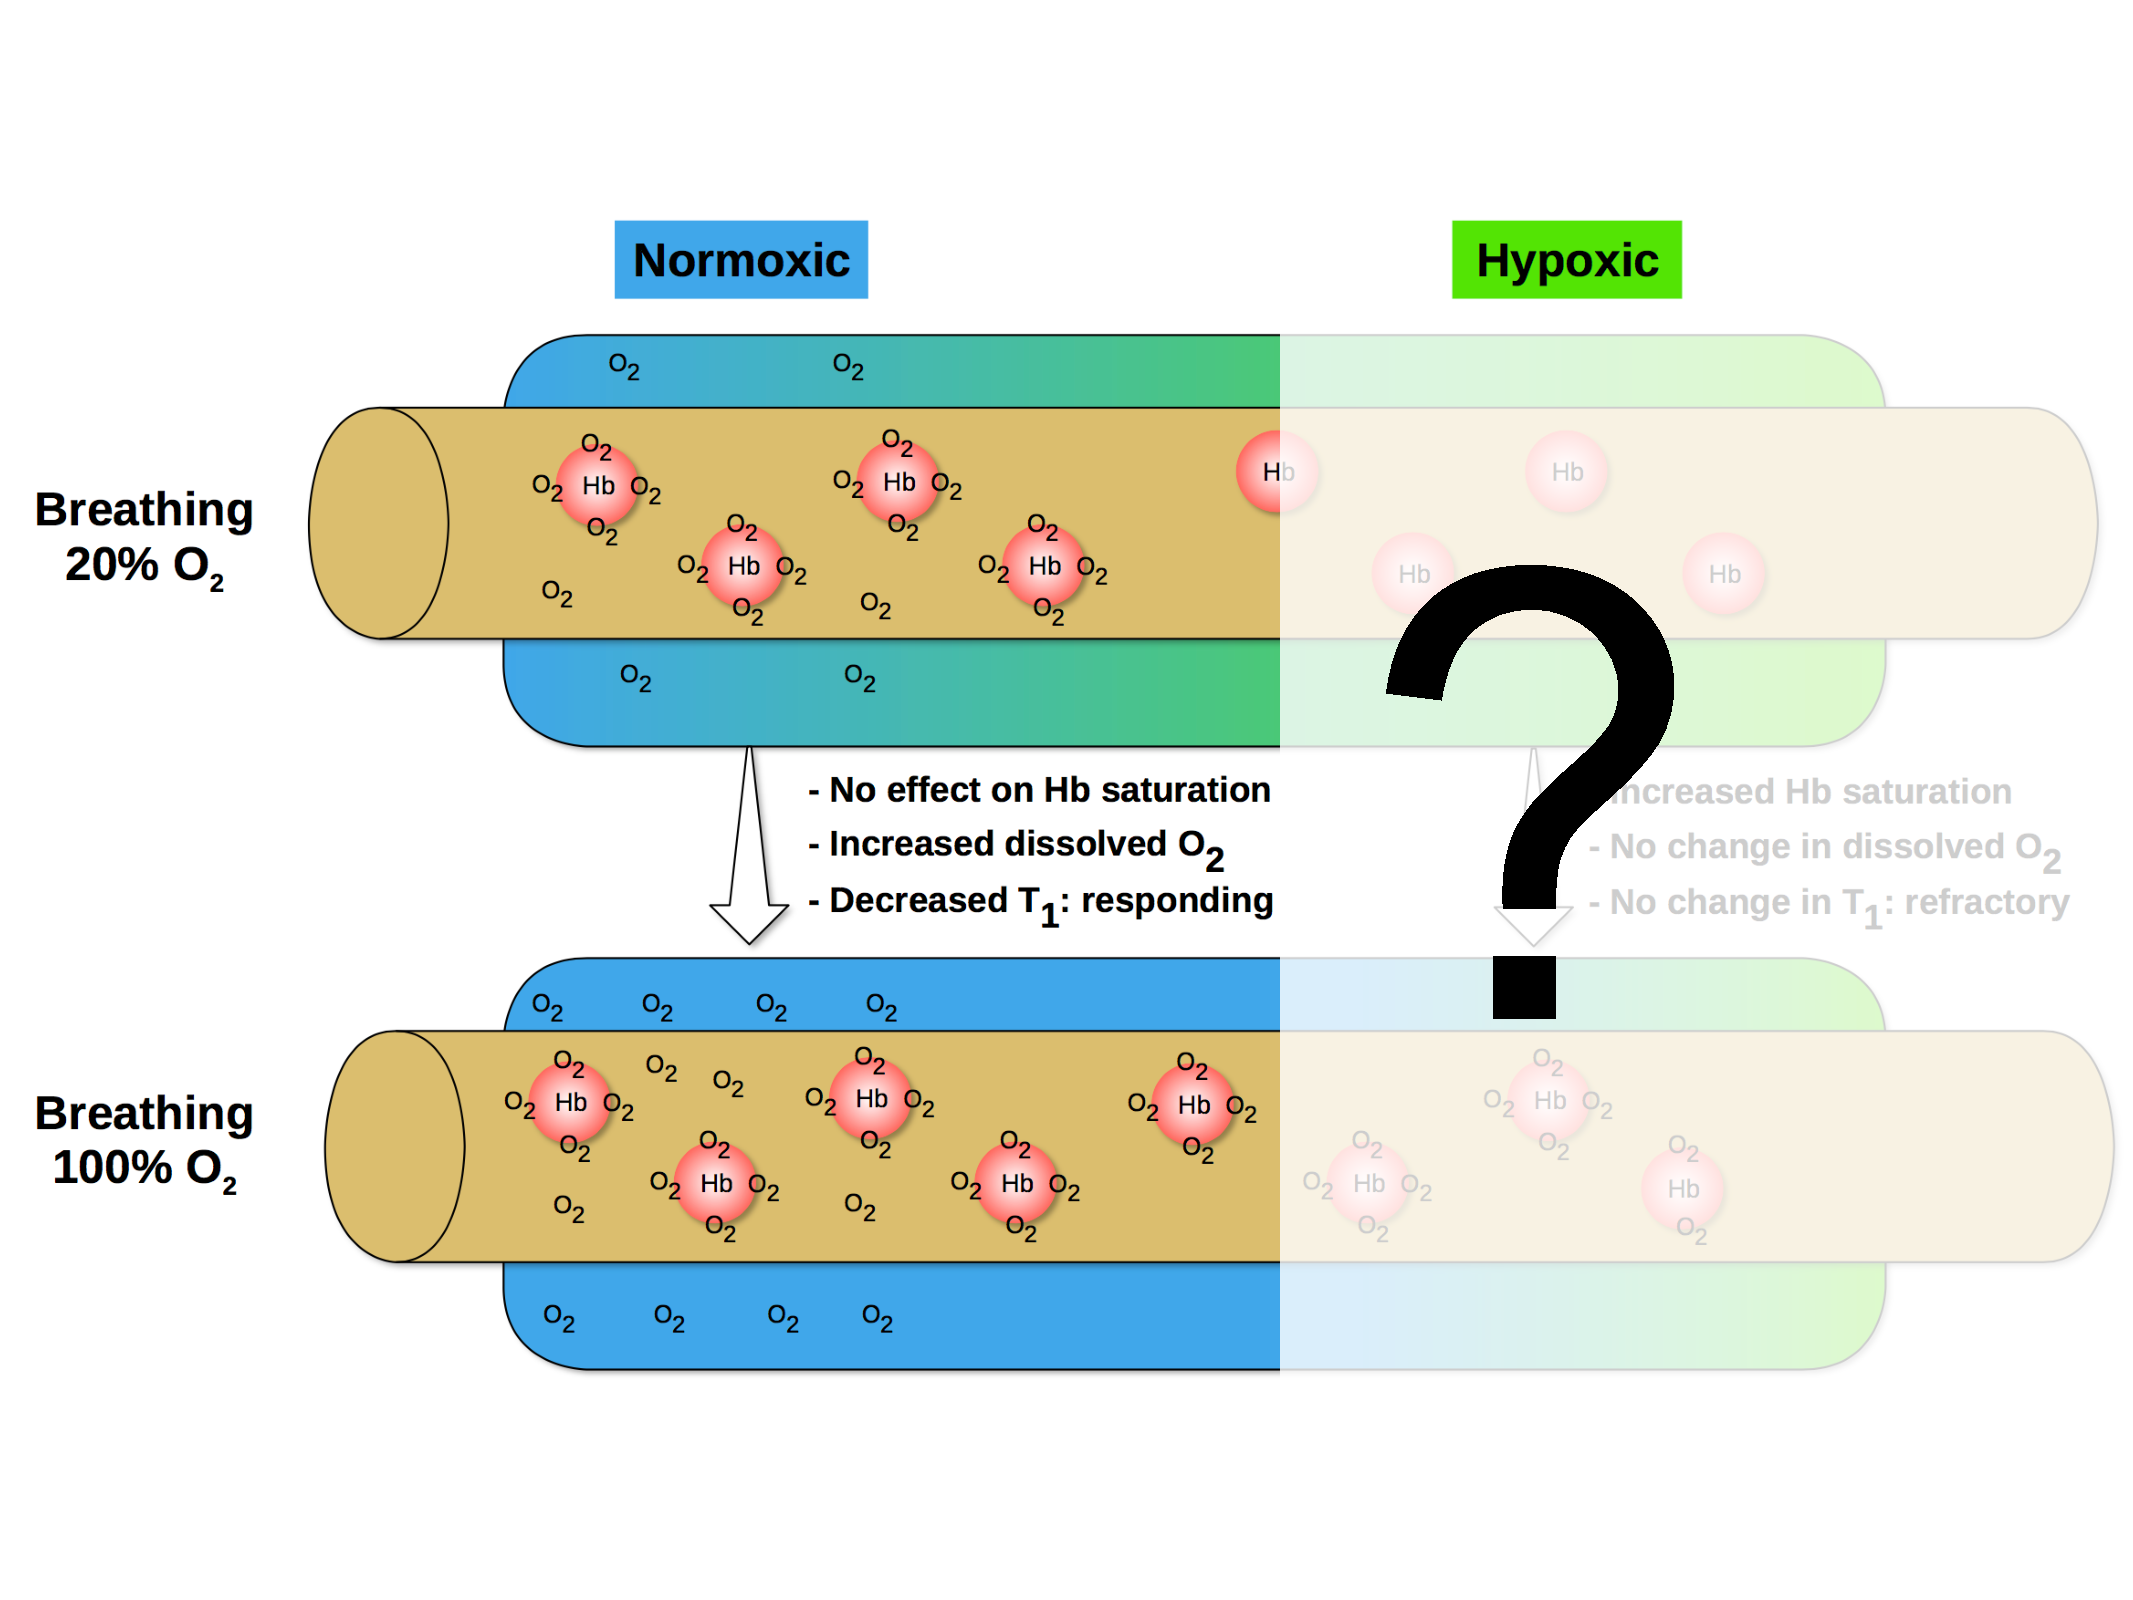
\includegraphics[width=\textwidth]{./intro/intro-images/oemriDark.pdf}
		\caption{A schematic representation of the origin of the OEMRI effect. In normoxic tissue, Hb is almost fully saturated and any excess breathed ${O_2}$ cannot bind to the Hb molecule. Consequently, ${O_2}$ dissolves in the blood plasma and as the excess oxygen diffuses out into the tissue, it also dissolves in the interstitial tissue fluid resulting in a net T$_1$ decrease. It is hypothesized that in the hypoxic tissue, Hb is not fully saturated with oxygen due to increased tissue demands and/or a poorly organized vascular network. The excess breathed oxygen in this case binds to the Hb molecule and does \textbf{not} dissolve in the plasma leading to no change in T$_1$.}
		\label{oemri}
		\end{center}
	\end{figure}

\section{Thesis structure}

In Chapter~\ref{ch:hpg} we begin by describing a new macromolecular contrast agent and explore its value in describing the tumour microenvironment.
A two-parameter linear model was applied to the contrast agent enhancement curve and we obtained measures of vessel permeability and fractional plasma volume.
These parameters were then used to distinguish between two tumour models.
In Chapter~\ref{ch:hpg2}, we applied this technique to determine whether molecule size played a role in the distribution of a high molecular weight anti-cancer drug (Trastuzumab).
Ultimately we showed that neither vessel permeability nor fractional plasma volume corresponded to presence of bound drug (determined via histological staining), suggesting other barriers that limit distribution of Trastuzumab.
In Chapter~\ref{ch:hpg3} we considered another application of the new contrast agent: can we assess changes in vessel permeability after administering an anti-angiogenic drug?
We discovered that vessel permeability is indeed reduced after drug treatment but along the way we also showed that histologically, hypoxia dramatically decreased after treatment. 
This led us along the journey to develop a new method to assess tumour oxygenation~\emph{in vivo} using MRI.
Chapter~\ref{ch:oemri} outlines the technique and how we used a blind source separation technique to increase sensitivity. 
We validated the technique in Chapter~\ref{ch:oemri2} with histological staining, and demonstrated utility of a new parameter to separate oxygenation replenishment in different tumour models.
Finally in Chapter~\ref{ch:oemri3} we showcase a typical application of the technique: detection of tumour oxygenation improvements after administering an anti-angiogenic agent. 
We also showed that the tumour implant site has a large bearing on the tumour microenviroment, and no oxygenation improvements are observed if the baseline oxygenation is high.
The thesis concludes with some interesting observations discovered that are worth future exploration and investigation.
